\documentclass[conference]{IEEEtran}
\IEEEoverridecommandlockouts
\usepackage[T1]{fontenc}
\usepackage{newtxtext,newtxmath}
\usepackage{graphicx}
\usepackage{booktabs}
\usepackage{multirow}
\usepackage{amsmath}
\usepackage{algorithm}
\usepackage{algpseudocode}
\usepackage{microtype}
\usepackage{cite}
\usepackage{xcolor}
\usepackage{balance}
\usepackage[hidelinks]{hyperref}
\graphicspath{{../figures/}}
\renewcommand{\algorithmicrequire}{\textbf{Input:}}
\renewcommand{\algorithmicensure}{\textbf{Output:}}
\newcommand{\Fone}{F\textsubscript{1}}

\begin{document}

\title{What Chronological Splits Expose in CICIDS2017: Label Artefacts, Duplicate Records and Cross-Dataset Failure in Flow-Based Intrusion Detection}

\makeatletter
\newcommand{\linebreakand}{\end{@IEEEauthorhalign}\hfill\mbox{}\par\mbox{}\hfill\begin{@IEEEauthorhalign}}
\makeatother
\author{
\IEEEauthorblockN{Anshveer Singh}
\IEEEauthorblockA{SCOPE\\
Vellore Institute of Technology\\
Vellore, India\\
anshveer.singh2023@vitstudent.ac.in}
\and
\IEEEauthorblockN{Gaurav Bakshi}
\IEEEauthorblockA{SCOPE\\
Vellore Institute of Technology\\
Vellore, India\\
gaurav.bakshi2023@vitstudent.ac.in}
\and
\IEEEauthorblockN{Dev Acharya Menon}
\IEEEauthorblockA{SCOPE\\
Vellore Institute of Technology\\
Vellore, India\\
dev.acharyamenon2023@vitstudent.ac.in}
\linebreakand
\IEEEauthorblockN{Anto S}
\IEEEauthorblockA{Associate Professor Sr., SCOPE\\
Vellore Institute of Technology\\
Vellore, India\\
anto.s@vit.ac.in}
}

\maketitle

\begin{abstract}
Flow-based intrusion detectors report near-perfect scores on CICIDS2017, and the gap to operational performance is usually attributed to leakage through duplicated or correlated records or to change in traffic over time. We test both explanations in one controlled pipeline that compares random, session-grouped, time-block-grouped and per-class chronological splits under a two-stage detector, which separates malicious from benign flows and then attributes each alert to an attack family. Exact-duplicate removal, grouping by flow identifier and grouping into 1--15 minute blocks change malicious-class \Fone{} by at most 0.004. A per-class chronological split lowers it from 0.997 to 0.903 and raises the benign false-positive rate from 0.07\% to 2.90\%. An audit of the false positives by endpoint and time shows that 98.8\% of them are benign-labelled flows between known attack endpoints: reverse-direction flows between the DDoS victim and the attacker address inside the 20-minute DDoS interval, and traffic from infected hosts to the Bot command-and-control server recorded after the last Bot-labelled flow. A random split places most of these flows in training and learns their labels; the chronological split places them in test. With them excluded from both protocols, the false-positive rates are equal (0.037\%) and the remaining difference is a recall loss (0.997 to 0.957), 85\% of it in DoS Hulk. We also report 309 feature vectors with conflicting labels, duplication concentrated in specific attacks, and the effect of scoring attribution end to end. Zero-shot transfer to CSE-CIC-IDS2018 on matched families collapses to a DoS recall of 0.0003, is unchanged without test-set deduplication and is not recovered by four label-free normalisations; unit identities hold, while 50 of 75 DoS-Hulk features shift with Kolmogorov--Smirnov statistic above 0.5.
\end{abstract}

\begin{IEEEkeywords}
intrusion detection, flow features, evaluation methodology, data leakage, label noise, temporal evaluation, dataset shift, CICIDS2017, CSE-CIC-IDS2018
\end{IEEEkeywords}

\section{Introduction}

Flow-level statistics such as packet-size moments, inter-arrival times and flag counts remain observable when payloads are encrypted, which makes flow-based classifiers a natural choice for detecting malicious activity in encrypted traffic \cite{anderson2016,anderson2017,drapergil2016}. Public benchmarks built with CICFlowMeter, most prominently CICIDS2017 \cite{sharafaldin2018} and CSE-CIC-IDS2018, report near-perfect accuracy for tree ensembles. Those numbers have repeatedly been questioned. Audits of CICIDS2017 have documented labelling errors, flow-construction artefacts and duplicated records \cite{engelen2021,liu2022,lanvin2023,rosay2022}, cross-dataset studies report that classifiers trained on one CIC dataset transfer poorly to the other \cite{cantone2024}, and general guidance on machine learning in security warns against random splits of temporally ordered data \cite{arp2022,pendlebury2019,sommer2010,kaufman2012}.

These lines of work leave two practical questions open. First, when a time-aware split lowers measured performance, how much of the drop is caused by leakage between near-identical records, and what is the rest? It is commonly read as change in traffic over time, which calls for temporal validation and model maintenance. On CICIDS2017, however, each attack occupies one short interval, so time-aware splits are usually built per class, and such a split does not test deployment after a fixed date. Its errors therefore have to be examined before they are attributed to drift. Second, attack attribution, i.e. naming the attack type behind an alert, is normally scored on ground-truth attack flows only, which ignores the errors of the detection stage that precedes it in any deployed system.

We address both questions with a controlled re-evaluation in which the data pipeline, features, model family and hyper-parameters are fixed and only one factor varies per comparison. The contributions are:
\begin{itemize}
\item A decomposition of the random-versus-chronological gap on CICIDS2017 into session leakage, adjacency leakage and the effect of per-class chronological ordering, using five split protocols built from the timestamped release of the dataset (Section~\ref{sec:splits}).
\item An endpoint and timing audit of the chronological-split false positives, which traces 98.8\% of them to benign-labelled flows of two attack sessions and shows that the false-positive gap disappears when these flows are excluded from both protocols (Section~\ref{sec:audit}).
\item A census of exact duplicates and label conflicts per attack class, and a sensitivity analysis of four duplicate-resolution policies on a common test set (Section~\ref{sec:integrity}).
\item An end-to-end evaluation of hierarchical attribution that quantifies how detection errors propagate into attack-family labels (Section~\ref{sec:hier}).
\item A matched-family transfer study from CICIDS2017 to CSE-CIC-IDS2018 with a same-year reference, a target-trained upper bound, the reverse direction, test-set deduplication controls, a diagnosis of the shift and an evaluation of label-free mitigations (Section~\ref{sec:cross}).
\end{itemize}
We position the study as a replication and extension of the cited audits and cross-dataset work: every comparison reports seed variability, and every claim is classified against an explicit noise floor.

\section{Related Work}

\textbf{Dataset construction and audits.} CICIDS2017 was generated from scripted benign profiles and attack schedules and processed with CICFlowMeter into roughly 80 flow features \cite{sharafaldin2018}. Engelen \textit{et al.} revisited its collection and found labelling and flow-construction problems \cite{engelen2021}; Liu \textit{et al.} extended the analysis to CSE-CIC-IDS2018, documented errors in attack orchestration, feature generation and labelling, and released corrected labelling logic \cite{liu2022}. Lanvin \textit{et al.} reported packet misordering, packet duplication and mislabelled attacks in CICIDS2017 and measured their effect on supervised detectors \cite{lanvin2023}; Rosay \textit{et al.} identified duplicated and miscalculated features and inconsistent TCP termination, leading to the corrected LycoS-IDS2017 dataset \cite{rosay2022}. Pekar and Jozsa compared detectors across original and refined versions of CICIDS2017 and observed that random forests remain accurate regardless of dataset integrity, which can hide data flaws \cite{pekar2024}. Ring \textit{et al.} survey network intrusion datasets more broadly \cite{ring2019}.

\textbf{Evaluation methodology.} Sommer and Paxson discussed why anomaly detection results in network security rarely transfer to operation \cite{sommer2010}. Arp \textit{et al.} catalogued pitfalls in security ML, including data snooping and sampling bias \cite{arp2022}, and Pendlebury \textit{et al.} showed that temporal and spatial bias inflate malware classifiers \cite{pendlebury2019}. Kaufman \textit{et al.} formalised leakage in data mining \cite{kaufman2012}. Most recently, Moczkodan and Ragab re-evaluated sequence models on CICIDS2017 and found that padding convention and split protocol dominate architectural choice, with leakage-free evaluation revealing a 67-fold increase in a Transformer's false-alarm rate \cite{moczkodan2026}. Apruzzese \textit{et al.} discussed practical assessment of ML-based network intrusion detection \cite{apruzzese2023}.

\textbf{Cross-dataset generalisation.} Cantone \textit{et al.} trained four classifiers on CIC-IDS-2017, CSE-CIC-IDS2018 and corrected variants and reported strong same-dataset results but poor transfer; for grouped binary detection from CIC-IDS-2017 to CSE-CIC-IDS2018 they report \Fone{} between 0.26 and 0.39 \cite{cantone2024}. On corrected data they also observed that some attacks were generated with different configurations in the two years.

\textbf{Encrypted-traffic classification.} Anderson and McGrew demonstrated malware detection from flow metadata and TLS context without decryption, and studied label noise and non-stationarity in that setting \cite{anderson2016,anderson2017}. Draper-Gil \textit{et al.} characterised encrypted and VPN traffic with time-related flow features \cite{drapergil2016}, and ET-BERT pre-trains Transformers on datagram representations \cite{lin2022}.

Table~\ref{tab:prior} places the present study relative to the closest prior work.

\begin{table}[t]
\centering
\caption{Closest prior work and the question each one leaves open}
\label{tab:prior}
\footnotesize
\setlength{\tabcolsep}{3pt}
\begin{tabular}{@{}p{0.26\columnwidth}p{0.33\columnwidth}p{0.35\columnwidth}@{}}
\toprule
Work & Focus & Open question addressed here \\
\midrule
Engelen \cite{engelen2021}, Liu \cite{liu2022}, Lanvin \cite{lanvin2023} & Label and capture errors, corrected data & Effect of feature-level label conflicts and dedup policy on reported metrics \\
Pekar \& Jozsa \cite{pekar2024} & Detector accuracy across data versions & Whether time-aware evaluation, rather than data integrity, drives the gap \\
Moczkodan \& Ragab \cite{moczkodan2026} & Sequence models, leakage-free splits & What the errors of a time-aware split consist of, for flow-level detectors and attribution \\
Cantone \textit{et al.} \cite{cantone2024} & Cross-dataset transfer & Same-year reference, upper bound, unit checks and mitigations on matched families \\
\bottomrule
\end{tabular}
\end{table}

\section{Data and Problem Setup}

\subsection{Datasets}
CICIDS2017 provides 2\,830\,743 labelled flows in eight capture files covering five working days; after removing records with missing or infinite values, 2\,827\,876 remain. Its \textit{MachineLearningCSV} release contains no timestamps, so we also use the \textit{GeneratedLabelledFlows} release, which carries flow identifiers and start timestamps. We verified that the two releases describe the same flows in the same order: flow duration, forward packet count and label agree on 100\% of rows in all eight files. Timestamps in the labelled release use a 12-hour clock without an AM/PM marker; because the capture covers working hours, hours below 8 were shifted by 12 hours (1\,471\,716 rows), after which all records fall between 08:42 and 17:10. CSE-CIC-IDS2018 contributes two days (16 and 22 February 2018) with 2\,097\,149 flows, of which 2\,091\,539 remain after the same cleaning; one repeated header row was removed.

\subsection{Features}
Identifiers and topology-dependent fields (flow identifier, IP addresses, ports, protocol, timestamp) and flow duration are excluded, leaving 76 statistics for CICIDS2017. The 2018 release abbreviates column names; an explicit alias table maps 2018 names to 2017 names, which yields 75 shared features (the 2017-only duplicate column \textit{Fwd Header Length.1} has no counterpart). Feature order is fixed by a single list and verified at prediction time.

\subsection{Labels and taxonomies}
Raw labels are canonicalised (for example, \textit{DoS attacks-Hulk} in 2018 maps to \textit{DoS Hulk}). Two attack taxonomies are used. The \emph{family} taxonomy has six attack classes: DoS/DDoS, PortScan, Brute Force (FTP and SSH Patator), Web Attack (brute force, XSS, SQL injection), Bot and Other/Rare (Infiltration, Heartbleed). The \emph{fine} taxonomy keeps every raw attack label with at least 500 records after deduplication as its own class and merges the remainder (SQL injection with 21 records, Infiltration with 36, Heartbleed with 11) into Other/Rare, which yields 12 attack classes.

\subsection{Notation}
Let $\mathcal{D}=\{(\mathbf{x}_i, y_i, t_i)\}_{i=1}^{N}$ with feature vector $\mathbf{x}_i\in\mathbb{R}^{d}$, raw label $y_i$ and start time $t_i$. A 64-bit hash $h(\mathbf{x})$ of the float32 feature vector defines duplicate groups $G_h=\{i : h(\mathbf{x}_i)=h\}$ and the conflict set
\begin{equation}
\mathcal{C}=\bigl\{h : |\{y_i : i\in G_h\}|\ge 2\bigr\}.
\end{equation}
A group in $\mathcal{C}$ contains flows that no deterministic classifier over these features can label correctly in full.

\section{Methodology}

\begin{figure*}[t]
\centering
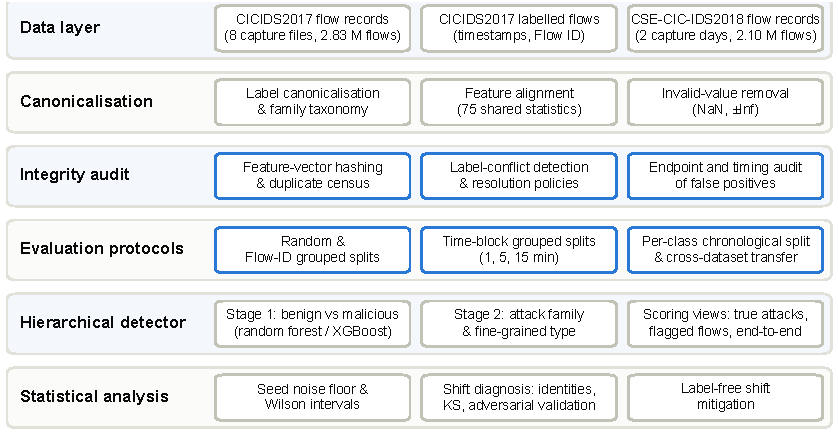
\includegraphics[width=0.95\textwidth]{fig_architecture}
\caption{Layered architecture of the evaluation system. Each layer consumes only the outputs of the layers above it; the integrity-audit and evaluation-protocol layers (outlined) are the components varied in the experiments.}
\label{fig:arch}
\end{figure*}

Fig.~\ref{fig:arch} shows the layered architecture. The canonicalisation layer produces aligned feature matrices; the integrity audit hashes every feature vector, records duplicates and conflicts and applies a resolution policy; the protocol layer generates train/test partitions; the detector layer trains and scores a two-stage model; and the analysis layer quantifies variability and dataset shift.

\subsection{Duplicate-resolution policies}
Four policies $\pi$ are compared: \emph{drop-conflicts} removes every group in $\mathcal{C}$ and keeps the first record of every other group (the default); \emph{keep-first} keeps the chronologically first record of every group regardless of label; \emph{majority} keeps one record per group labelled with the group's most frequent label; \emph{none} keeps all records. For the sensitivity study the split is assigned per hash group \emph{before} a policy is applied, so that every policy sees the same partition of groups and no exact duplicate can cross the split. Each policy is scored on its own test population and on a \emph{common} test set made of conflict-free test groups, one record each, which is identical across policies.

\subsection{Evaluation protocols}
\label{sec:protocols}
All splits are stratified by raw label with a test fraction of 0.2, so every attack class appears in training and test. For a class $\ell$ with $n_\ell$ records:
\begin{itemize}
\item \emph{Random}: uniform stratified sampling.
\item \emph{Flow-ID grouped}: records sharing a flow identifier (addresses, ports and protocol) form a group; groups are permuted and moved to the test side until at least $0.2\,n_\ell$ records are covered, leaving at least one group in training.
\item \emph{Time-block grouped}: records are grouped by $b_i=\lfloor t_i/(60W)\rfloor$ with $W\in\{1,5,15\}$ minutes and assigned as above. Blocks are interleaved in time, so the test blocks of a class lie between its training blocks.
\item \emph{Chronological (timestamps)}: records of class $\ell$ are ordered by $t_i$; the latest $n_\ell-\lfloor 0.8\,n_\ell\rfloor$ form the test set and the $\lfloor 0.01\,n_\ell\rfloor$ records immediately preceding the cut (for $n_\ell\ge 100$) are purged.
\item \emph{Chronological (row order)}: the same rule applied to capture-file row order, the only ordering available in the timestamp-free release.
\end{itemize}
Each class is cut at its own time; there is no global cutoff. Training flows of one class can therefore be later than test flows of another: 86\% of chronological test flows have at least one later training flow, and 103\,694 of the 265\,566 attack training flows (39\%; DDoS, PortScan and Bot) were recorded inside the period covered by the benign test flows, Thursday 16:23 to Friday 17:02. A single global cutoff is not feasible on this dataset because each attack occupies one interval of minutes to hours: for cutoffs at the 50th to 90th percentiles of capture time at most two of the 14 attack classes have flows on both sides, and a cutoff at the start of Friday leaves none. The comparison random $\rightarrow$ grouped isolates leakage between correlated records; grouped $\rightarrow$ chronological isolates the effect of testing each class on the end of its own capture interval. The chronological splits are therefore not a simulation of deployment on a future period.

\subsection{Hierarchical detector}
Stage 1 is a binary classifier $f_1:\mathbb{R}^d\rightarrow\{0,1\}$ trained on all training flows; Stage 2 is a family (or fine-type) classifier $f_2$ trained on malicious training flows only. The deployed prediction is
\begin{equation}
\hat{y}(\mathbf{x})=\begin{cases} f_2(\mathbf{x}) & \text{if } f_1(\mathbf{x})=1,\\ \text{Benign} & \text{otherwise.}\end{cases}
\end{equation}
Attribution is scored in three views: on ground-truth malicious flows (isolating $f_2$), on flows flagged by $f_1$ (where benign false positives receive an attack label by construction), and end to end over all test flows. Both stages are random forests \cite{breiman2001} with 100 trees, maximum depth 20 and balanced class weights; a gradient-boosted alternative \cite{chen2016} (300 trees, depth 6, learning rate 0.1, histogram method, positive-class weight equal to the class ratio) is used as a robustness check. Tree ensembles are invariant to monotone feature scaling, so no scaler is fitted.

\subsection{Statistical treatment}
Model randomness is measured by repeating each configuration over seeds; for random and grouped splits the seed controls both the partition and the model, while the two chronological splits are deterministic and the seed controls the model only. Macro-\Fone{} averages per-class \Fone{} with equal weight; the benign false-positive rate is $\mathrm{FPR}=\mathrm{FP}/(\mathrm{FP}+\mathrm{TN})$ over benign test flows. Proportions $\hat p=k/n$ carry Wilson 95\% intervals \cite{wilson1927},
\begin{equation}
\frac{\hat p+\frac{z^2}{2n}\pm z\sqrt{\frac{\hat p(1-\hat p)}{n}+\frac{z^2}{4n^2}}}{1+\frac{z^2}{n}},\qquad z=1.96 .
\end{equation}
The model-seed standard deviation of family macro-\Fone{} under the row-order chronological split ($\sigma=0.013$, five seeds) is the largest among headline metrics and serves as the noise floor. A difference $\Delta$ between configurations $a$ and $b$ is called material when $|\Delta|>\max\bigl(0.013,\;2\sqrt{s_a^2+s_b^2}\bigr)$, with the second term applied only when both sides have several seeds. No multiple-comparison correction is applied, and we do not report significance tests.

\subsection{Endpoint audit of false positives}
\label{sec:auditmethod}
Addresses and ports are never used as features, but the labelled release retains them, which allows false positives to be inspected. For the timestamp chronological split and the random split (seed 42), the models are re-fitted with identical settings, the stored confusion counts are reproduced exactly, and every benign test flow predicted malicious is grouped by source address, destination address, destination port and hour. Two endpoint sets emerge from the chronological-split false positives (Section~\ref{sec:audit}): $A_1$, flows between the DDoS victim 192.168.10.50 and the attacker address 172.16.0.1, and $A_2$, flows to or from the Bot command-and-control (C\&C) address 205.174.165.73 on port 8080. For a test set with benign subset $\mathcal{B}$, the audited false-positive rate is
\begin{equation}
\mathrm{FPR}_A=\frac{\bigl|\{i\in\mathcal{B}\setminus A : f_1(\mathbf{x}_i)=1\}\bigr|}{|\mathcal{B}\setminus A|},\qquad A=A_1\cup A_2,
\end{equation}
applied identically to both protocols; precision, recall and \Fone{} are recomputed with $\mathcal{B}\cap A$ removed, and attack-labelled flows are never removed. Because the sets were identified from the errors they explain, the audited metrics describe what those errors consist of; they are not a corrected benchmark.

\begin{algorithm}[t]
\caption{Leakage-aware hierarchical evaluation}
\label{alg:eval}
\begin{algorithmic}[1]
\Require flows $\mathcal{D}$, policy $\pi$, protocol $P$, seeds $S$
\Ensure per-view metrics with seed variability
\State $\mathcal{D}\gets \textsc{Clean}(\mathcal{D})$ \Comment{drop NaN/$\pm\infty$}
\State compute $h(\mathbf{x}_i)$, groups $G_h$, conflict set $\mathcal{C}$
\State $\mathcal{D}_\pi\gets \textsc{Resolve}(\mathcal{D},\mathcal{C},\pi)$
\For{$s\in S$}
  \State $(\mathcal{T}_r,\mathcal{T}_e)\gets P(\mathcal{D}_\pi, s)$ \Comment{per-label 80/20}
  \State assert feature order of $\mathcal{T}_e$ equals that of $\mathcal{T}_r$
  \State train $f_1$ on $\mathcal{T}_r$; train $f_2$ on $\{(\mathbf{x},y)\in\mathcal{T}_r : y\neq\text{Benign}\}$
  \State score $f_1$: malicious \Fone, precision, recall, benign FPR
  \State score $f_2$ on true attacks, on flagged flows, end to end
\EndFor
\State \Return mean, SD and range over $S$; Wilson intervals per class
\end{algorithmic}
\end{algorithm}

\subsection{Cross-dataset protocol and shift diagnosis}
The transfer study restricts both datasets to the families present in the two 2018 days: Benign, DoS/DDoS and Web Attack. Models are trained on the training partition of the CICIDS2017 row-order chronological split, restricted to these families, and scored (i) on the matching CICIDS2017 test partition, as a same-year reference, and (ii) on all deduplicated 2018 flows. The target-trained upper bound uses the same per-class rule on the 2018 data. Three diagnostics probe the shift.

\textit{Unit identities.} If duration $D$ is in microseconds and rates are per second, the CICFlowMeter definitions imply
\begin{equation}
\label{eq:units}
\begin{gathered}
\frac{D\,R_b}{B_f+B_b}=10^6,\qquad \frac{D\,R_p}{P_f+P_b}=10^6,\\
\frac{\mu_{\mathrm{IAT}}\,(P_f+P_b-1)}{D}=1,
\end{gathered}
\end{equation}
where $B$ and $P$ are byte and packet totals, $R_b$ and $R_p$ the byte and packet rates and $\mu_{\mathrm{IAT}}$ the mean inter-arrival time. A unit change between tool versions would violate these ratios in one dataset.

\textit{Per-feature shift.} For each feature and matched class, the two-sample Kolmogorov--Smirnov statistic $D_{\mathrm{KS}}=\sup_x|\hat F_{2017}(x)-\hat F_{2018}(x)|$ is computed on 100\,000-row samples per year.

\textit{Adversarial validation.} A random forest is trained to distinguish 2017 from 2018 records; its held-out area under the ROC curve measures joint separability \cite{quionero2009}.

Four transformations that use no 2018 labels are then evaluated: a signed logarithm $\operatorname{sgn}(x)\log(1+|x|)$; per-dataset robust scaling $(x-\mathrm{med}_d)/\mathrm{IQR}_d$; per-dataset quantile mapping $\hat F_d(x)$; and removal of the $k\in\{10,25\}$ features with the largest $D_{\mathrm{KS}}$ between 2017 training data and unlabelled 2018 data. Statistics for 2018 are computed on all unlabelled 2018 flows, so these transformations are transductive. Their effect is summarised by the share of the transfer gap they recover,
\begin{equation}
G(T)=\frac{F_{\mathrm{cross}}(T)-F_{\mathrm{cross}}(\varnothing)}{F_{\mathrm{ref}}(\varnothing)-F_{\mathrm{cross}}(\varnothing)},
\end{equation}
with $F$ the end-to-end macro-\Fone{} and $\varnothing$ the untransformed features.

\begin{algorithm}[t]
\caption{Shift diagnosis and label-free mitigation}
\label{alg:shift}
\begin{algorithmic}[1]
\Require source $\mathcal{D}_{17}$, target $\mathcal{D}_{18}$, shared families $\mathcal{F}$
\State align features by alias table; map labels to $\mathcal{F}$
\For{class $c\in\{\text{Benign},\text{DoS Hulk}\}$ and year}
  \State verify unit identities \eqref{eq:units} on $D>0$ records
\EndFor
\State $D_{\mathrm{KS}}(j,c)$ for every feature $j$ and class $c$
\State adversarial AUC for (all), (Benign), (DoS Hulk)
\For{$T\in\{\varnothing,\text{slog},\text{robust},\text{quantile},\text{drop}_{10},\text{drop}_{25}\}$}
  \State fit $T$ on $\mathcal{D}_{17}^{\mathrm{train}}$ and on unlabelled $\mathcal{D}_{18}$ separately
  \State train $f_1,f_2$ on $T(\mathcal{D}_{17}^{\mathrm{train}})$
  \State score on $T(\mathcal{D}_{17}^{\mathrm{test}})$ and $T(\mathcal{D}_{18})$; compute $G(T)$
\EndFor
\end{algorithmic}
\end{algorithm}

\section{Results}

\subsection{Data integrity}
\label{sec:integrity}

Of the 2\,827\,876 valid CICIDS2017 records, 2\,198\,624 are unique feature vectors (22.25\% exact duplicates). The conflict set contains 309 vectors covering 82\,704 rows; the largest single group holds 6\,654 rows. Every conflicting vector is labelled benign in at least one occurrence. By label, 158 conflicting vectors involve DoS Hulk, 106 PortScan, 40 Bot, 3 DDoS and 2 slowloris; PortScan's 76\,265 conflicting rows therefore stem from only 106 distinct vectors. After conflict removal and deduplication, 2\,198\,315 records remain.

Duplication is far from uniform across classes (Fig.~\ref{fig:dup}). In CICIDS2017, 98.8\% of PortScan rows are duplicates (158\,804 rows, 1\,956 unique vectors), against 0.0\% for DDoS. In the two 2018 days, DoS-SlowHTTPTest consists of 55 unique vectors in 139\,890 rows, one of which accounts for 44.3\% of the class, consistent with the repetition reported for corrected 2018 data \cite{cantone2024}. Probing attacks emit nearly identical flows, so deduplication removes most of exactly those classes and reshapes the evaluated class mix.

\begin{figure*}[t]
\centering
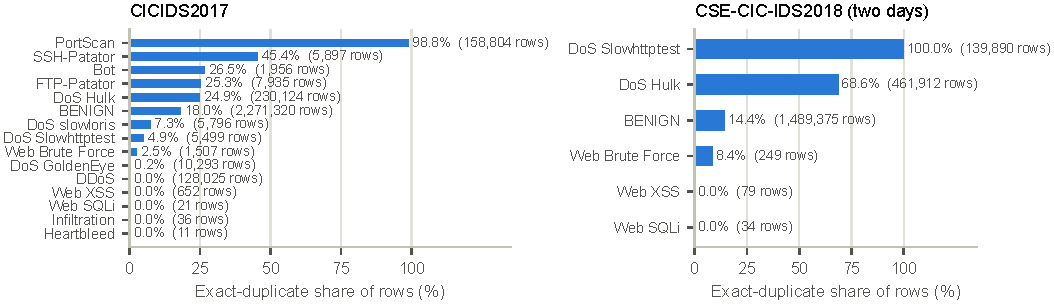
\includegraphics[width=0.95\textwidth]{fig_duplication}
\caption{Share of rows that are exact feature-vector duplicates, per raw label, before any resolution policy. Row counts in parentheses.}
\label{fig:dup}
\end{figure*}

Table~\ref{tab:dedup} reports the policy study. On the common test set, all four policies agree within 0.001 malicious \Fone{} under the random group split and within 0.004 under the row-order chronological split. Under the chronological split, family macro-\Fone{} on true attacks varies between $-0.014$ and $+0.025$ around the default policy, which is one to two seed standard deviations and, with a single seed per policy, not interpretable. A naive row-level random split without deduplication leaves an exact duplicate in training for 24.85\% of test rows, yet changes malicious \Fone{} by only $+0.0014$ relative to a hash-group split; what changes is the test population, with PortScan support growing from 370 to 31\,761 rows.

\begin{table}[t]
\centering
\caption{Duplicate-resolution policies (random forest, one seed)}
\label{tab:dedup}
\footnotesize
\setlength{\tabcolsep}{3.2pt}
\begin{tabular}{@{}llrccc@{}}
\toprule
Split & Policy / test set & $n_{\text{test}}$ & Mal.\ \Fone & FPR (\%) & Fam.\ \Fone \\
\midrule
\multirow{5}{*}{Random} & drop-conflicts / common & 439\,665 & 0.9966 & 0.077 & 0.975 \\
 & keep-first / common & 439\,665 & 0.9967 & 0.078 & 0.974 \\
 & majority / common & 439\,665 & 0.9965 & 0.081 & 0.974 \\
 & none / common & 439\,665 & 0.9968 & 0.082 & 0.975 \\
 & none, row split / own & 565\,576 & 0.9968 & 0.124 & 0.965 \\
\midrule
\multirow{4}{*}{\shortstack[l]{Chron.\\(rows)}} & drop-conflicts / common & 439\,721 & 0.9003 & 3.041 & 0.842 \\
 & keep-first / common & 439\,721 & 0.9012 & 2.934 & 0.866 \\
 & majority / common & 439\,721 & 0.8999 & 3.013 & 0.828 \\
 & none / common & 439\,721 & 0.9034 & 2.988 & 0.867 \\
\bottomrule
\end{tabular}
\end{table}

\subsection{Leakage versus chronological ordering}
\label{sec:splits}

Fig.~\ref{fig:splits} and Table~\ref{tab:splits} compare the five protocols. Grouping by flow identifier leaves every headline metric unchanged within noise ($\Delta$ malicious \Fone{} $=-0.0002$). Time-block grouping lowers malicious \Fone{} by 0.001--0.004 and keeps family attribution within noise for 1- and 5-minute blocks; fine-grained attribution loses 0.017--0.060. Moving from interleaved blocks to the timestamp chronological split lowers malicious \Fone{} by 0.089--0.092, family macro-\Fone{} on true attacks by 0.116--0.133 and end-to-end family macro-\Fone{} by 0.113--0.153. The five-seed replication under row order confirms the size of the effect: malicious \Fone{} $0.9029\pm0.0033$ against $0.9966\pm0.0000$, family macro-\Fone{} $0.838\pm0.013$ against $0.974\pm0.000$.

\begin{figure*}[t]
\centering
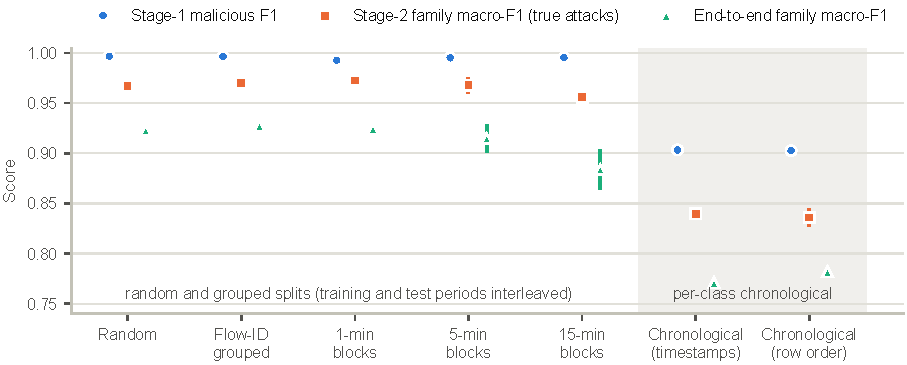
\includegraphics[width=0.95\textwidth]{fig_splits}
\caption{Detection and attribution under five split protocols (CICIDS2017, drop-conflicts policy, random forest). Markers show the mean over two seeds and vertical lines the range. Grouped splits remove correlated records from the test side but interleave training and test periods; only the shaded protocols test each class on the end of its own capture interval.}
\label{fig:splits}
\end{figure*}

\begin{table}[t]
\centering
\caption{Split protocols (mean of 2 seeds; row order with 5 seeds in parentheses)}
\label{tab:splits}
\footnotesize
\setlength{\tabcolsep}{2.0pt}
\begin{tabular}{@{}lccccc@{}}
\toprule
Protocol & Mal.\ \Fone & Prec. & Recall & FPR (\%) & Fam.\ \Fone{} (GT) \\
\midrule
Random & 0.9966 & 0.9963 & 0.9969 & 0.067 & 0.967 \\
Flow-ID grouped & 0.9965 & 0.9959 & 0.9970 & 0.074 & 0.970 \\
1-min blocks & 0.9927 & 0.9958 & 0.9897 & 0.085 & 0.973 \\
5-min blocks & 0.9953 & 0.9974 & 0.9933 & 0.065 & 0.968 \\
15-min blocks & 0.9954 & 0.9984 & 0.9924 & 0.103 & 0.956 \\
Chron., timestamps & 0.9033 & 0.8562 & 0.9559 & 2.899 & 0.840 \\
Chron., row order & 0.9026 & 0.8551 & 0.9556 & 2.922 & 0.836 \\
\quad (5 seeds) & (0.9029) & (0.8553) & (0.9562) & (2.922) & (0.838) \\
\bottomrule
\end{tabular}
\end{table}

The chronological-split decline is mainly a precision effect. Precision falls from 0.996 to 0.856 and recall from 0.997 to 0.956, while the benign FPR rises from 0.067\% to 2.90\%, about 44-fold in the five-seed comparison (2.92\% against 0.066\%). Holding recall at its random-split value, the observed precision alone would give \Fone{} $=0.921$; holding precision, the observed recall alone would give $0.976$. Section~\ref{sec:audit} examines the false positives. Recall losses are class specific (Fig.~\ref{fig:recall}): DoS Hulk falls from 0.997 to 0.927, slowloris from 0.997 to 0.899 and SSH-Patator from 0.978 to 0.781, while DDoS and FTP-Patator are unaffected. DoS Hulk, whose test flows cover the last 11 minutes of its 24-minute attack interval, accounts for 85\% of the missed attack flows in both seeds (2\,465 of 2\,896 for seed 42). PortScan differs from the overall pattern: its recall already falls from 0.993 to 0.830 under 5-minute grouping and stays at 0.826 under the chronological split, so its random-split score is explained by adjacency between near-identical probe flows.

\begin{figure}[t]
\centering
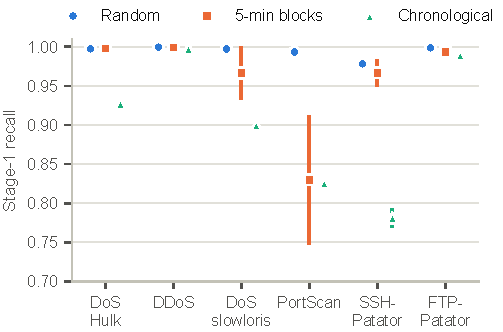
\includegraphics[width=\columnwidth]{fig_class_recall}
\caption{Stage-1 recall per attack under three protocols (mean and range over two seeds).}
\label{fig:recall}
\end{figure}

The timestamped release also tests whether capture-file row order is a valid proxy for time. Row order is chronological in the five Thursday and Friday files (Spearman $\rho\approx1.00$) but not in the Monday, Tuesday and Wednesday files ($\rho=0.48$, $0.47$ and $0.66$). Nevertheless the row-order and timestamp chronological splits share 86\% of their test flows and differ by at most 0.011 on any headline metric, which is within noise; per-class recall can still differ (SSH-Patator 0.912 against 0.781).

\subsection{What the chronological false positives are}
\label{sec:audit}

Table~\ref{tab:audit} and Fig.~\ref{fig:fp} report the endpoint audit of Section~\ref{sec:auditmethod}. Of the 10\,612 benign false positives of the timestamp chronological split (seed 42), 9\,685 (91.3\%) lie on the attacker--victim pair $A_1$ and 802 (7.6\%) on the Bot C\&C channel $A_2$; 125 lie elsewhere.

\textit{Attacker--victim pair.} All but 3 of the 128\,011 DDoS-labelled flows run from the attacker address to the victim, and every DDoS test flow is addressed to port 80. The 9\,680 benign flows that Stage 2 labels DDoS run in the opposite direction, from the victim to ports at or above 1024 of the attacker address (99.97\%), and 9\,681 of them were recorded inside the labelled DDoS interval, 15:56--16:16 on Friday. Inside that interval the benign FPR is 20.5\%; outside it, 0.26\%. These flows share endpoints and time with the attack and differ from it only in direction, which is consistent with the flow-construction and labelling defects reported for this dataset \cite{engelen2021,lanvin2023}.

\textit{Bot C\&C channel.} Of the 803 benign flows labelled Bot by Stage 2, 802 go from five internal hosts to 205.174.165.73 on port 8080, the hosts, address and port of all 280 Bot-labelled test flows. The last Bot-labelled flow was recorded at 12:59 on Friday; all but one of the 803 were recorded between 13:00 and 17:00, so the C\&C channel continues after the Bot label ends.

\begin{table}[t]
\centering
\caption{Endpoint audit of benign false positives (seed 42)}
\label{tab:audit}
\footnotesize
\setlength{\tabcolsep}{3pt}
\begin{tabular}{@{}lrr@{}}
\toprule
 & Random & Chronological \\
\midrule
Benign test flows & 372\,431 & 372\,432 \\
\quad on attacker--victim pair $A_1$ & 7\,620 & 31\,515 \\
\quad on Bot C\&C channel $A_2$ & 179 & 966 \\
Benign false positives & 254 & 10\,612 \\
\quad on $A_1$ & 4 & 9\,685 \\
\quad on $A_2$ & 116 & 802 \\
\quad elsewhere & 134 & 125 \\
\midrule
FPR, all benign flows (\%) & 0.068 & 2.849 \\
FPR$_A$, $A=A_1\cup A_2$ removed (\%) & 0.037 & 0.037 \\
Precision / recall, $A$ removed & 0.998 / 0.997 & 0.998 / 0.957 \\
Malicious \Fone{}, all / $A$ removed & 0.997 / 0.997 & 0.905 / 0.977 \\
\bottomrule
\end{tabular}
\end{table}

\begin{figure}[t]
\centering
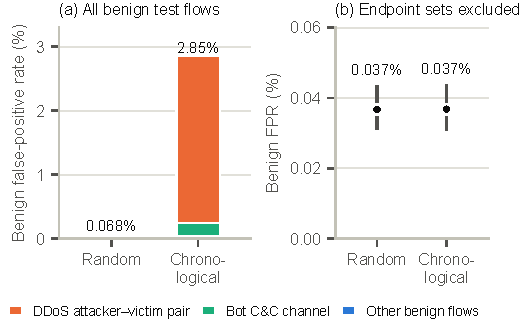
\includegraphics[width=\columnwidth]{fig_fp}
\caption{Benign false-positive rate of the random and timestamp chronological splits (seed 42). (a) All benign test flows, divided by the endpoint set on which each false positive lies. (b) After removing benign flows on both endpoint sets from both test sets; lines show Wilson 95\% intervals.}
\label{fig:fp}
\end{figure}

\textit{Mechanism.} The random split places about 80\% of these flows in training under their benign labels, and the model learns them: of 7\,620 benign test flows on $A_1$ only 4 are false positives. The chronological split places all of them in test, because they are the latest benign flows, while the matching attack flows remain in training. The five row-order seeds show the same composition: flows assigned to DDoS make up 90.8--91.9\% of benign false positives, against 2.6--5.2\% under random splits.

\textit{After the audit.} With $\mathcal{B}\cap A$ removed from both test sets (32\,481 chronological and 7\,799 random benign test flows), the FPR is 0.037\% under both protocols, with Wilson interval $[0.031,\,0.044]\%$ in both cases, and precision is 0.998 for both. Malicious \Fone{} is 0.977 against 0.997: the gap falls from 0.092 to 0.020, which still exceeds the noise floor and consists entirely of the recall difference (0.957 against 0.997). Whether the remaining DoS-Hulk recall loss reflects a change in the attack tool's behaviour or another labelling effect was not examined.

\subsection{Hierarchical attribution}
\label{sec:hier}

Scoring attribution only on true attacks overstates what an analyst would see (Fig.~\ref{fig:hier}). Under the random split, Bot attribution has \Fone{} 0.996 on true attacks and 0.729 end to end (precision 0.664, recall 0.818), even though the benign FPR is only 0.066\%: with 280 Bot test flows, the share of the 246 benign false positives that Stage 2 assigns to Bot is enough to lower its precision by a third, and for seed 42 all 116 benign flows assigned to Bot lie on the C\&C channel $A_2$. Under the row-order chronological split the end-to-end Bot \Fone{} falls to 0.411 with precision 0.259, and DoS/DDoS falls from 0.990 to 0.898; Section~\ref{sec:audit} identifies these false positives as the benign-labelled flows on $A_2$ and $A_1$. End-to-end scoring therefore exposes label defects as well as detector errors. Within the web-attack family, brute force and cross-site scripting are hard to separate from flow statistics even under the random split (fine \Fone{} $0.723\pm0.003$ and $0.459\pm0.014$), which supports scoring them as one family. Slow-rate denial-of-service attacks are separable under the random split (slowloris \Fone{} 0.995) but not under the chronological split (0.735).

\begin{figure}[t]
\centering
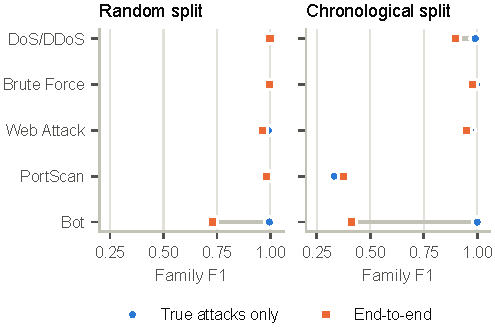
\includegraphics[width=\columnwidth]{fig_hierarchy}
\caption{Family \Fone{} of Stage 2 scored on true attacks only and end to end through Stage 1 (five seeds).}
\label{fig:hier}
\end{figure}

\subsection{Cross-dataset transfer}
\label{sec:cross}

Table~\ref{tab:cross} and Fig.~\ref{fig:cross} summarise the transfer study. The same models that reach end-to-end macro-\Fone{} $0.949\pm0.003$ on the CICIDS2017 reference reach $0.322\pm0.015$ on 2018. DoS recall is $0.0003\pm0.0002$ on 145\,254 flows and web-attack recall $0.011\pm0.024$ on 335 flows (Wilson interval $[0,\,0.011]$ for seed 42). Almost every 2018 flow is labelled benign (Fig.~\ref{fig:cm}). Scoring every 2018 row without deduplication does not change the conclusion: malicious \Fone{} is $0.0087\pm0.0078$ and SlowHTTPTest recall is 0.000 over all 139\,890 of its rows. The failure is symmetric, as a model trained on 2018 and tested on the matching CICIDS2017 classes reaches end-to-end macro-\Fone{} 0.337 and DoS recall 0.031 (one seed). Gradient boosting also fails (DoS recall 0.000, one seed). A model trained and tested on 2018 reaches DoS recall 1.000, web-attack recall $0.765\pm0.029$ on 68 test flows and benign FPR 0.0016\%, so the 75 features are sufficient within each year.

\begin{table}[t]
\centering
\caption{Matched-family transfer (random forest; mean $\pm$ SD over seeds)}
\label{tab:cross}
\footnotesize
\setlength{\tabcolsep}{1.9pt}
\begin{tabular}{@{}lccccc@{}}
\toprule
Train $\rightarrow$ test & Seeds & E2E \Fone & DoS rec. & Web rec. & FPR (\%) \\
\midrule
2017 $\rightarrow$ 2017 & 5 & $0.949\pm0.003$ & 0.943 & 0.937 & 2.588 \\
2017 $\rightarrow$ 2018 & 5 & $0.322\pm0.015$ & 0.0003 & 0.011 & 0.013 \\
2017 $\rightarrow$ 2018, no dedup & 3 & $0.280\pm0.003$ & 0.0044 & 0.000 & 0.011 \\
2018 $\rightarrow$ 2018 & 3 & $0.949\pm0.010$ & 1.000 & 0.765 & 0.002 \\
2018 $\rightarrow$ 2017 & 1 & 0.337 & 0.031 & 0.000 & 0.503 \\
\bottomrule
\end{tabular}
\end{table}

\begin{figure}[t]
\centering
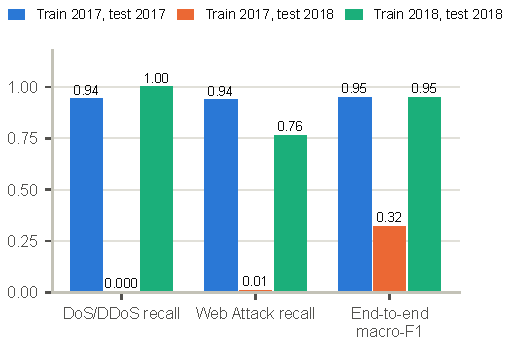
\includegraphics[width=\columnwidth]{fig_cross}
\caption{Matched-family recall and end-to-end macro-\Fone{} for the same-year reference, zero-shot transfer and a target-trained model.}
\label{fig:cross}
\end{figure}

\begin{figure}[t]
\centering
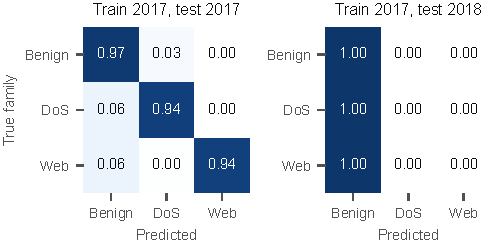
\includegraphics[width=\columnwidth]{fig_confusion}
\caption{Row-normalised end-to-end confusion matrices, seed 42. In 2018, 145\,169 of 145\,254 DoS flows and all 335 web-attack flows are labelled benign.}
\label{fig:cm}
\end{figure}

The diagnostics locate the shift. The unit identities \eqref{eq:units} hold in both years for benign and DoS-Hulk flows, with medians equal to $1.000\times10^6$, $1.000\times10^6$ and $1.000$ to three significant figures, which excludes a change of measurement units between tool versions. The years are nonetheless jointly separable: adversarial validation reaches AUC 0.9997 on all records and 0.9997 on benign records alone, driven by header lengths, the minimum forward segment size and minimum inter-arrival times. The magnitude of the shift differs sharply by class (Fig.~\ref{fig:shift}). For DoS Hulk, 50 of 75 features have $D_{\mathrm{KS}}>0.5$, with a maximum of 0.911; for benign traffic none exceeds 0.445. The most shifted DoS-Hulk features describe the backward direction: 82.3\% of 2018 Hulk flows carry no backward payload against 9.5\% in 2017, the median backward initial window changes from 235 to $-1$, the value recorded when no backward window is observed, and the median flow duration falls from 86.4\,s to 0.051\,s. Within 2017, the feature that best separates Hulk from benign traffic is the mean backward packet length (importance 0.128 in a classifier trained to distinguish the two), so a 2018 Hulk flow without a backward response lacks the evidence that separates the classes in the training year.

\begin{figure}[t]
\centering
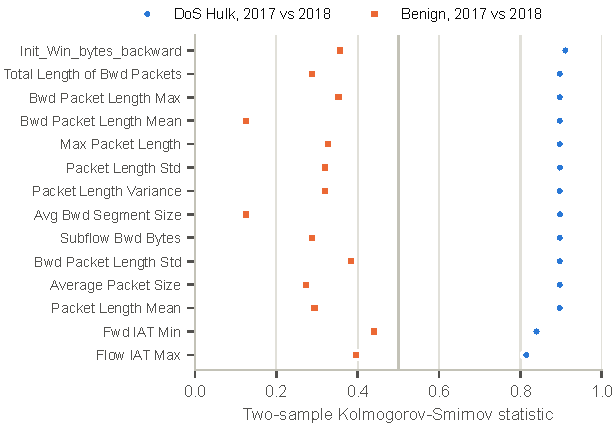
\includegraphics[width=\columnwidth]{fig_shift}
\caption{Kolmogorov--Smirnov statistic between years for the 14 most shifted DoS-Hulk features, with the benign statistic for the same features. The vertical line marks $D_{\mathrm{KS}}=0.5$.}
\label{fig:shift}
\end{figure}

None of the label-free transformations closes the gap (Fig.~\ref{fig:mitig}). With random forests over three seeds, the recovered share $G(T)$ is 0.0\% for the signed logarithm, 0.0\% for robust scaling, $-0.2\%$ for quantile mapping and 0.5\% and 0.1\% when the 10 or 25 most shifted features are removed; robust scaling drives all 2018 predictions to benign and quantile mapping raises the 2018 benign FPR to 0.71\% without detecting any DoS flow. Gradient boosting with the 10 most shifted features removed recovers 15.5\% and reaches web-attack recall 0.29, but with one seed and DoS recall 0.000. The globally most shifted features are forward-direction and timing statistics dominated by the benign majority of 2018 traffic; the backward-direction features that carry the DoS-Hulk shift rank between 35th and 46th and were never removed. Removing class-specific shifted features would require 2018 labels and was not attempted.

\begin{figure}[t]
\centering
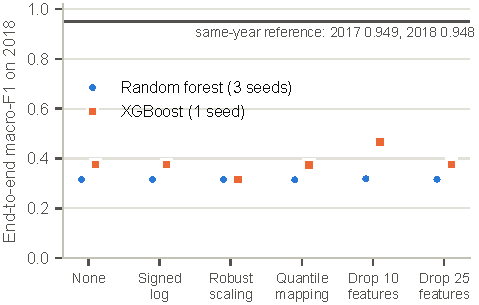
\includegraphics[width=\columnwidth]{fig_mitigation}
\caption{End-to-end macro-\Fone{} on 2018 after label-free transformations. Random-forest markers show the mean of three seeds and lines the range.}
\label{fig:mitig}
\end{figure}

\section{Discussion}

\textbf{What inflates the benchmark.} Exact duplicates, session-level correlation and minute-scale adjacency together account for at most 0.004 malicious \Fone{} on CICIDS2017. Deduplication remains necessary for a correct test population, and PortScan shows that adjacency leakage can dominate an individual class, but none of these explains a large share of the reported performance. This agrees with Pekar and Jozsa's observation that random forests are robust to data-integrity defects \cite{pekar2024}.

\textbf{What a chronological split measures.} The per-class chronological split costs 0.09 \Fone{} and multiplies false positives by about 44, which would ordinarily be read as temporal drift. The audit shows that 98.8\% of those false positives are benign-labelled flows of two attack sessions, which a random split learns from training data and a chronological split moves into the test set. On this dataset the split therefore acts mainly as an audit of labels: it makes memorised label defects visible as errors. After the audit the false-positive rates coincide, and the residual effect is a recall loss of 0.040 concentrated in one attack. A time-aware split should accordingly be reported together with an inspection of its errors before any part of the drop is attributed to drift. Whether the false-alarm increases reported for other time-aware protocols on CICIDS2017 \cite{moczkodan2026} have the same composition is untested.

\textbf{Attribution.} A hierarchical system inherits its detector's false positives. Reporting Stage-2 quality on true attacks alone hides failures that are visible at the first triage step, such as the drop of Bot \Fone{} from 1.00 to 0.41; on CICIDS2017 these failures include label defects, which end-to-end scoring exposes.

\textbf{Transfer.} Our transfer result is more severe than the grouped binary \Fone{} of 0.26--0.39 reported by Cantone \textit{et al.} for the same direction \cite{cantone2024}. Deduplication does not explain the difference (Table~\ref{tab:cross}). Our 2018 test set covers DoS Hulk, SlowHTTPTest and web attacks only, while theirs covers all attack days; the attack-subset explanation is plausible but was not tested. The diagnostics show that DoS-Hulk traffic of the two years differs strongly on the backward-direction features that separate Hulk from benign traffic in 2017, while benign traffic differs much less. This is consistent with the different attack configurations Cantone \textit{et al.} observed on corrected data, but the diagnostics are correlational: they do not establish which features cause the failure. They do explain why matching marginal distributions without labels cannot restore detection.

\textbf{Recommendations.} Report a time-aware split alongside any random split, state whether its cutoff is global or per class, and audit its false positives by endpoint and time; publish the benign FPR with its denominator; report duplicate and conflict counts per class and the resolution policy; score attribution end to end; and accompany cross-dataset results with a same-year reference and a target-trained upper bound.

\textbf{Threats to validity.} The chronological splits cut each class at its own time and do not simulate deployment after a fixed date (Section~\ref{sec:protocols}); a global cutoff is not feasible on CICIDS2017. The endpoint sets were identified from the errors they explain, so the audited metrics are a post-hoc diagnostic of one seed per protocol, supported by the five-seed share of DDoS-assigned false positives; the affected flows were not relabelled. The protocol comparison uses two seeds per split; the policy study, the reverse transfer and gradient boosting use one seed; and seeds on deterministic splits measure model randomness only. The study uses one dataset pair and two 2018 days, so the transfer analysis covers three attack labels. Labels are otherwise taken from the public releases, whose errors are documented elsewhere \cite{engelen2021,liu2022,lanvin2023}. Only tree ensembles were evaluated.

\section{Conclusion}

On CICIDS2017, duplicated and correlated records account for at most 0.004 of malicious-class \Fone{}. A per-class chronological split lowers \Fone{} by 0.09 and raises false positives about 44-fold, but 98.8\% of those false positives are benign-labelled flows between known attack endpoints that a random split learns from its training data. With these flows excluded identically from both protocols, the false-positive rates coincide and the gap falls to a recall difference of 0.040, mostly in DoS Hulk. The chronological gap on this dataset is therefore mainly a label artefact, not evidence of temporal drift. Label conflicts, class-specific duplication and end-to-end attribution scoring change which numbers a study reports. Zero-shot transfer to CSE-CIC-IDS2018 fails; unit checks exclude a change of measurement units, the diagnostics are consistent with a change in the attack traffic, and label-free normalisation does not repair it. Future work should relabel the affected flows and repeat the protocol comparison, extend the transfer analysis to all 2018 attack days, test class-aware adaptation with a small labelled target sample, and evaluate the same protocols on encrypted-traffic captures with TLS metadata.

\balance
\begin{thebibliography}{99}
\footnotesize
\bibitem{sharafaldin2018} I. Sharafaldin, A. H. Lashkari, and A. A. Ghorbani, ``Toward generating a new intrusion detection dataset and intrusion traffic characterization,'' in \textit{Proc. 4th Int. Conf. Information Systems Security and Privacy (ICISSP)}, 2018, pp. 108--116.
\bibitem{engelen2021} G. Engelen, V. Rimmer, and W. Joosen, ``Troubleshooting an intrusion detection dataset: the CICIDS2017 case study,'' in \textit{Proc. IEEE Security and Privacy Workshops (SPW)}, 2021, doi: 10.1109/SPW53761.2021.00009.
\bibitem{liu2022} L. Liu, G. Engelen, T. Lynar, D. Essam, and W. Joosen, ``Error prevalence in NIDS datasets: A case study on CIC-IDS-2017 and CSE-CIC-IDS-2018,'' in \textit{Proc. IEEE Conf. Communications and Network Security (CNS)}, 2022, pp. 254--263.
\bibitem{lanvin2023} M. Lanvin, P.-F. Gimenez, Y. Han, F. Majorczyk, L. M\'e, and \'E. Totel, ``Errors in the CICIDS2017 dataset and the significant differences in detection performances it makes,'' in \textit{Risks and Security of Internet and Systems (CRiSIS 2022)}, LNCS, Springer, 2023, pp. 18--33.
\bibitem{rosay2022} A. Rosay, E. Cheval, F. Carlier, and P. Leroux, ``Network intrusion detection: A comprehensive analysis of CIC-IDS2017,'' in \textit{Proc. 8th Int. Conf. Information Systems Security and Privacy (ICISSP)}, 2022.
\bibitem{pekar2024} A. Pekar and R. Jozsa, ``Evaluating ML-based anomaly detection across datasets of varied integrity: A case study,'' \textit{Computer Networks}, 2024, arXiv:2401.16843.
\bibitem{cantone2024} M. Cantone, C. Marrocco, and A. Bria, ``On the cross-dataset generalization of machine learning for network intrusion detection,'' \textit{IEEE Access}, vol. 12, pp. 144489--144508, 2024.
\bibitem{moczkodan2026} Z. Moczkodan and H. Ragab, ``Do transformers actually help intrusion detection? A temporal sequence evaluation on CIC-IDS2017,'' arXiv:2606.11098, 2026.
\bibitem{arp2022} D. Arp, E. Quiring, F. Pendlebury, A. Warnecke, F. Pierazzi, C. Wressnegger, L. Cavallaro, and K. Rieck, ``Dos and don'ts of machine learning in computer security,'' in \textit{Proc. 31st USENIX Security Symp.}, 2022.
\bibitem{pendlebury2019} F. Pendlebury, F. Pierazzi, R. Jordaney, J. Kinder, and L. Cavallaro, ``TESSERACT: Eliminating experimental bias in malware classification across space and time,'' in \textit{Proc. 28th USENIX Security Symp.}, 2019.
\bibitem{sommer2010} R. Sommer and V. Paxson, ``Outside the closed world: On using machine learning for network intrusion detection,'' in \textit{Proc. IEEE Symp. Security and Privacy}, 2010, pp. 305--316.
\bibitem{kaufman2012} S. Kaufman, S. Rosset, C. Perlich, and O. Stitelman, ``Leakage in data mining: Formulation, detection, and avoidance,'' \textit{ACM Trans. Knowledge Discovery from Data}, vol. 6, no. 4, 2012.
\bibitem{apruzzese2023} G. Apruzzese, P. Laskov, and J. Schneider, ``SoK: Pragmatic assessment of machine learning for network intrusion detection,'' in \textit{Proc. IEEE European Symp. Security and Privacy (EuroS\&P)}, 2023.
\bibitem{ring2019} M. Ring, S. Wunderlich, D. Scheuring, D. Landes, and A. Hotho, ``A survey of network-based intrusion detection data sets,'' \textit{Computers \& Security}, vol. 86, pp. 147--167, 2019.
\bibitem{anderson2016} B. Anderson and D. McGrew, ``Identifying encrypted malware traffic with contextual flow data,'' in \textit{Proc. ACM Workshop on Artificial Intelligence and Security (AISec)}, 2016, pp. 35--46.
\bibitem{anderson2017} B. Anderson and D. McGrew, ``Machine learning for encrypted malware traffic classification: Accounting for noisy labels and non-stationarity,'' in \textit{Proc. 23rd ACM SIGKDD Int. Conf. Knowledge Discovery and Data Mining}, 2017, pp. 1723--1732.
\bibitem{drapergil2016} G. Draper-Gil, A. H. Lashkari, M. S. I. Mamun, and A. A. Ghorbani, ``Characterization of encrypted and VPN traffic using time-related fea\-tures,'' in \textit{Proc. 2nd Int. Conf. Information Systems Security and Privacy (ICISSP)}, 2016, pp. 407--414.
\bibitem{lin2022} X. Lin, G. Xiong, G. Gou, Z. Li, J. Shi, and J. Yu, ``ET-BERT: A contextualized datagram representation with pre-training transformers for encrypted traffic classification,'' in \textit{Proc. ACM Web Conf. (WWW)}, 2022, pp. 633--642.
\bibitem{breiman2001} L. Breiman, ``Random forests,'' \textit{Machine Learning}, vol. 45, no. 1, pp. 5--32, 2001.
\bibitem{chen2016} T. Chen and C. Guestrin, ``XGBoost: A scalable tree boosting system,'' in \textit{Proc. 22nd ACM SIGKDD Int. Conf. Knowledge Discovery and Data Mining}, 2016, pp. 785--794.
\bibitem{wilson1927} E. B. Wilson, ``Probable inference, the law of succession, and statistical inference,'' \textit{J. American Statistical Association}, vol. 22, no. 158, pp. 209--212, 1927.
\bibitem{quionero2009} J. Qui\~nonero-Candela, M. Sugiyama, A. Schwaighofer, and N. D. Lawrence, Eds., \textit{Dataset Shift in Machine Learning}. Cambridge, MA, USA: MIT Press, 2009.
\end{thebibliography}

\end{document}
